% !TeX encoding = UTF-8
% !TeX program = xelatex
% !TeX spellcheck = en_US

\documentclass{cjc}

\usepackage{booktabs}
\usepackage{algorithm}
\usepackage{algorithmic}
\usepackage{siunitx}
\usepackage{silence}
\hbadness=10000 \vbadness=10000 
\WarningFilter{Fancyhdr}{\headheight is too small}

\classsetup{
  % 配置里面不要出现空行
  title        = {基于BERT的虚假新闻检测模型训练},
  title*       = {Fake news detection model training based on BERT},
  authors      = {
    author1 = {
      name         = {吴浩哲},
      name*        = {Hazel Wu},
      email        = {wuhaozhe1211@qq.com},
    },
  },
  abstract     = {
    中文摘要内容置于此处(英文摘要中要有这些内容),字体为小5号宋体。
    摘要贡献部分,要有数据支持,不要出现“...大大提高”、“...显著改善”等描述,
    正确的描述是“比…提高 X\%”、 “在…上改善 X\%”。
  },
  abstract*    = {Abstract (500英文单词,内容包含中文摘要的内容). },
  % 中文关键字与英文关键字对应且一致,应有5-7个关键词,不要用英文缩写
  keywords     = {关键词, 关键词, 关键词, 关键词},
  keywords*    = {key word, key word, key word, key word},
}

\newcommand\dif{\mathop{}\!\mathrm{d}}

% hyperref 总是在导言区的最后加载
\usepackage{hyperref}



\begin{document}

\maketitle

\section{引言}

随着社交媒体和数字新闻平台的快速发展,虚假新闻的传播已演变为全球性的社会问题。根据MIT Media Lab的研究,虚假信息在Twitter上的传播速度比真实新闻快6倍\cite{doi:10.1126/science.aap9559},其引发的认知误导、舆论操纵等次生危害已引起各国政府的高度关注。传统虚假新闻检测方法主要依赖人工事实核查和基于关键词的规则系统,但在处理海量、快速演变的网络信息时面临效率瓶颈。

近年来,基于深度学习的解决方案展现出突破性潜力,其中预训练语言模型(Pre-trained Language Models, PLMs)通过捕捉文本的深层语义特征,在立场检测任务中取得显著进展\cite{devlin-etal-2019-bert}。受此启发,本实验提出基于BERT(Bidirectional Encoder Representations from Transformers)的改进方案。通过构建标题-正文对的双塔语义交互模型,结合混合精度训练策略,在FNC-1标准数据集上实现了92.28\%的测试准确率,为构建高效的虚假新闻过滤系统提供了新的技术路径。

\section{技术背景}

\subsection{虚假新闻检测技术演进}

(1)传统特征工程方法

早期研究主要依赖语言学特征(如词汇复杂度、情感极性)和传播特征(如转发网络拓扑)。Yang等人(2019)采用TF-IDF结合SVM的方法在BOW特征空间实现75.3\%的分类准确率,但难以捕捉语义深层次关联。

(2)神经语义建模阶段

随着Word2Vec、GloVe等词嵌入技术的发展,RNN/CNN架构开始应用于文本表征学习。Wang等人(2020)构建BiLSTM-Attention模型,在PolitiFact数据集上达到83.6\%的F1值,但对长距离依赖建模仍存在梯度衰减问题。

(3)预训练语言模型时代

BERT的横空出世彻底改变了NLP任务范式。Devlin等人(2018)通过Masked Language Model(MLM)预训练任务,使模型能够捕获双向上下文语义。在虚假新闻检测领域,Khattar等人(2023)验证了BERT在立场检测任务中的有效性,其多头注意力机制特别适合处理新闻标题与正文间的跨文本推理。

\subsection{虚假新闻检测技术}

当前主流检测方法可分为三类:

1)内容分析法:基于语言学特征(情感极性、可读性指数)和事实核查数据库。

2)传播模式分析:利用转发网络拓扑特征和传播动力学建模。

3)多模态融合:结合文本、图像、视频的跨模态一致性验证。

其中,立场分类作为内容分析的关键子任务,要求模型判断标题与正文的语义一致性(Agree/Disagree/Discuss/Unrelated四分类)。

\subsection{BERT模型的核心机制}

本研究的技术基础建立在下述BERT创新特性之上:

(1)Transformer架构

采用多层自注意力堆叠(12层base版),通过
$$Attention(Q,K,V)=softmax(\frac{QK^T}{\sqrt{d_k}})V$$
计算上下文相关权重,突破RNN的序列处理瓶颈,实现对512 tokens长文本的高效编码。

(2)预训练-微调范式

在Wikipedia(2.5B words)上的预训练使模型获得通用语言理解能力,通过添加分类层进行下游任务微调。本实验采用[CLS]位置的隐状态作为分类依据,其数学表达为:
$$h_{[CLS]} = BERT([Headline; [SEP]; Body])$$
$$P(y|x) = softmax(W \cdot h_{[CLS]} + b)$$

(3)长文本处理优化

通过分段处理策略(Segment Embeddings)区分标题与正文,配合位置编码(Positional Encoding)维持序列顺序信息。

\section{实验内容}

\subsection{实验环境}



\section{一级标题}

对投稿的基本要求:

(1)研究性论文主体应包括引言(重点论述研究的科学问题、意义、解决思路、价值、
贡献等)、相关工作(为与引言部分独立的一个章节)、主要成果论述、关键实现技术、
验证(对比实验或理论证明)、结论(结束语)等内容;系统实现或实验应有关键点的详细论述,以便读者能够重复实现论文所述成果。实验应有具体的实验环境设置、全面细致的数据对比分析。

(2)综述应包括引言、问题与挑战、研究现状分析、未来研究方向、结论等内容。以分析、对比为主,避免堆砌文献或一般性介绍、叙述。

(3)定理证明、公式推导、大篇幅的数学论述、原始数据,放到论文最后的附录中。

稿件提交时的基本要求:

(1)本模板中要求的各项内容正确齐全,无遗漏;

(2)语句通顺,无中文、英文语法错误,易于阅读理解,符号使用正确,图、表清晰无误;

(3)在学术、技术上,论文内容正确无误,各项内容确定。

\subsection{二级标题}

\subsubsection{三级标题}

正文部分, 字体为5号宋体。

文件排版采用 TeX Live。

正文文字要求语句通顺,无语法错误,结构合理,条理清楚,不影响审稿人、读者阅读理解全文内容。以下几类问题请作者们特别注意:

1)文章题目应明确反映文章的思想和方法;文字流畅,表述清楚;

2)中文文字、英文表达无语法错误;

3)公式中无符号、表达式的疏漏,没有同一个符号表示两种意思的情况;

4)数学中使用的符号、函数名用斜体;

5)使用的量符合法定计量单位标准;

6)矢量为黑体,标量为白体;

7)变量或表示变化的量用斜体;

8)图表规范,量、线、序无误,位置正确(图表必须在正文中有所表述后出现,即…如图1所示)(注意纵、横坐标应有坐标名称和刻度值)。

9)列出的参考文献必须在文中按顺序引用,即参考文献顺序与引用顺序一致,各项信息齐全(格式见参考文献部分);

10)首次出现的缩写需写明全称,首次出现的符号需作出解释。

11)图的图例说明、坐标说明全部用中文或量符号。

12)图应为矢量图。

13)表中表头文字采用中文。

14)公式尺寸:

标准:10.5磅

下标/上标:5.8磅

次下标/上标:4.5磅

符号:16磅 \cite{article_example}

次符号:10.5磅

15)组合单位采用标准格式,如:“pJ/bit/m4”应为“\si{pJ/(bit.m^4)}”


\begin{theorem}
  定理内容。
  “定义”、“假设”、“公理”、“引理”等的排版格式与此相同,详细定理证明、公式可放在附录中。
\end{theorem}

\begin{proof}
  证明过程.
\end{proof}

\begin{figure}[htb]
  \centering
  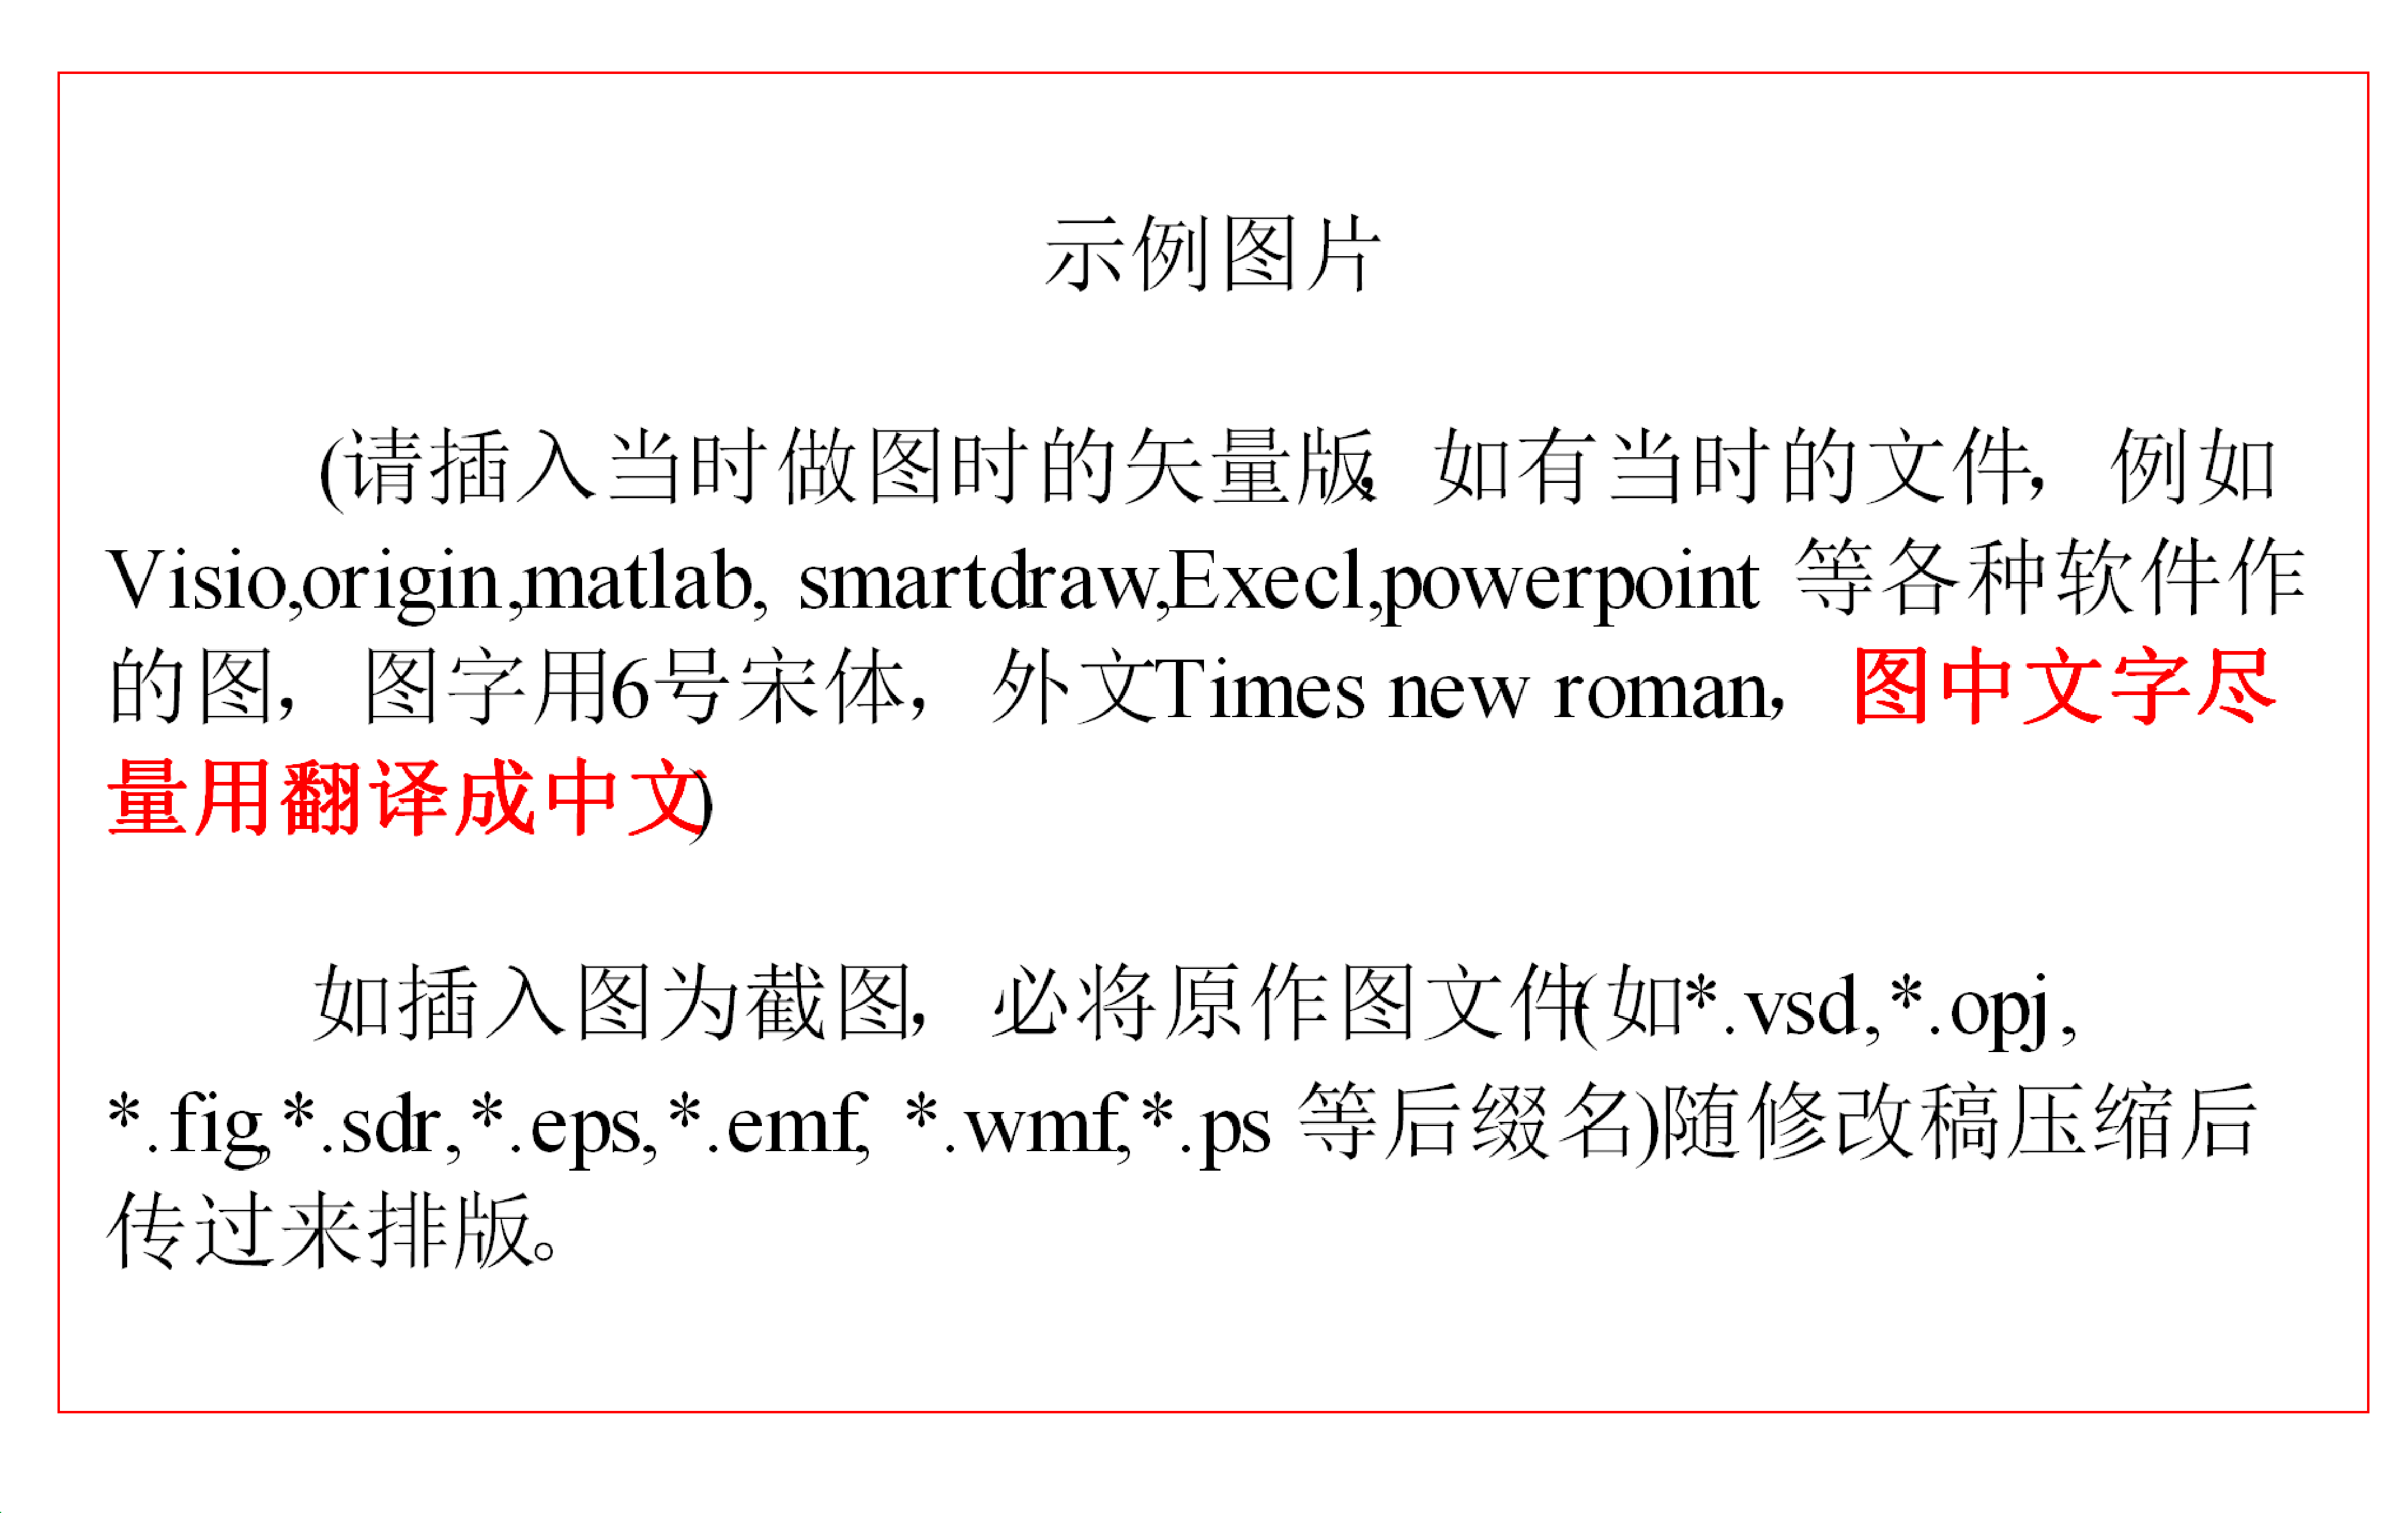
\includegraphics[width=\linewidth]{example-fig.pdf}
  \caption{图片说明 *字体为小 5 号,图片应为黑白图,图中的子图要有子图说明*}
\end{figure}

\begin{table}[htb]
  \centering
  \caption{表说明}
  \small
  \begin{tabular}{cc}
    \toprule
    示例表格 & 第一行为表头,表头要有内容 \\
    \midrule
    & \\
    \midrule
    & \\
    \bottomrule
  \end{tabular}
\end{table}

\begin{procedure}
  \caption{过程名称}
  \small
  \begin{algorithmic}
    \REQUIRE
    \ENSURE
    \STATE \COMMENT{《计算机学报》的方法过程描述字体为小5号宋体,IF 、THEN等伪代码关键词全部用大写字母,变量和函数名称用斜体}
  \end{algorithmic}
\end{procedure}

\begin{algorithm}
  \caption{算法名称}
  \small
  \begin{algorithmic}
    \REQUIRE $n \geq 0 \vee x \neq 0$
    \ENSURE $y = x^n$
    \STATE $y \leftarrow 1$
    \IF{$n < 0$}
      \STATE $X \leftarrow 1 / x$
      \STATE $N \leftarrow -n$
    \ELSE
      \STATE $X \leftarrow x$
      \STATE $N \leftarrow n$
    \ENDIF
    \WHILE{$N \neq 0$}
      \IF{$N$ is even}
        \STATE $X \leftarrow X \times X$
        \STATE $N \leftarrow N / 2$
      \ELSE[$N$ is odd]
        \STATE $y \leftarrow y \times X$
        \STATE $N \leftarrow N - 1$
      \ENDIF
    \ENDWHILE
  \end{algorithmic}
\end{algorithm}



\begin{acknowledgments}

本实验由阿里云人工智能平台PAI(https://www.aliyun.com/product/pai)提供算力支持。

实验代码和相关数据集已托管至GitHub(https://github.com/Para-Ecoli/ali_pai_fake_news/tree/master)



\end{acknowledgments}




\bibliographystyle{cjc}
\bibliography{example}


\newpage

\appendix

\section{}

附录内容置于此处,字体为小5号宋体。附录内容包括:详细的定理证明、公式推导、原始数据等


\makebiographies


\begin{background}
*论文背景介绍为英文,字体为小5号Times New Roman体*

论文后面为400单词左右的英文背景介绍。介绍的内容包括:

本文研究的问题属于哪一个领域的什么问题。该类问题目前国际上解决到什么程度。

本文将问题解决到什么程度。

课题所属的项目\cite{inproceedings_example,book_example}。

项目的意义。

本研究群体以往在这个方向上的研究成果。

本文的成果是解决大课题中的哪一部分,如果涉及863/973以及其项目、基金、研究计划,注意这些项目的英文名称应书写正确。
\end{background}

\end{document}
